\begin{figure}[!htbp]
	\centering
	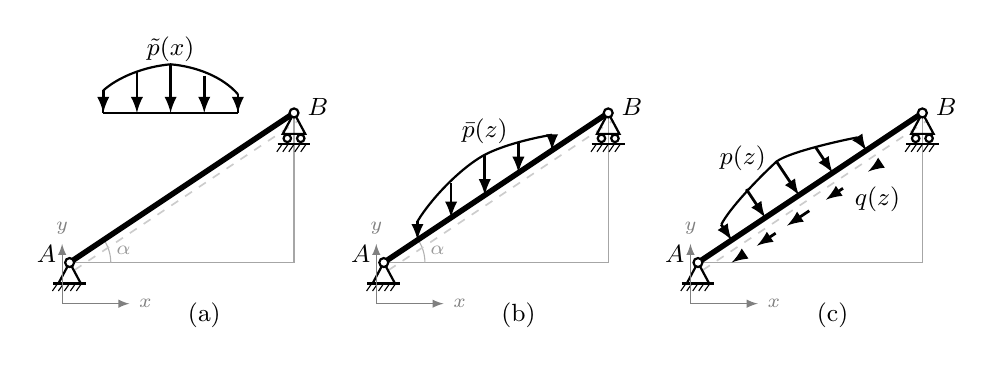
\begin{tikzpicture}[
		scale=0.95,
		>=latex,
		axis/.style={->, thin, gray},
		trave/.style={line width=2pt},
		carico/.style={line width=1pt}, trattcarico/.style={line width=1pt}, 
		pcomp/.style={line width=1pt},
		qcomp/.style={line width=1pt},
		tratt/.style={gray!70, thin}, 
		fibre/.style={dashed, gray!40, line width=0.6pt},
		]
		]
		
		% ── Parametri dei vincoli (convenzione C06/C07) ──
		\def\tw{0.15}    % semi-larghezza triangolo
		\def\thR{0.28}   % altezza triangolo
		\def\rn{0.06}    % raggio anellino (perno)
		\def\rw{0.05}    % raggio ruote del carrello
		\def\bw{0.09}    % semi-distanza ruote
		\def\gw{0.22}    % semi-larghezza barra di terra
		\def\hh{0.10}    % profondità del tratteggio del suolo
		
		
		% =========================================================
		% PANNELLO (a)
		% =========================================================
		\begin{scope}[xshift=0cm]
			
			\draw[trattcarico] (0.45,2) -- (2.25,2);
			%\draw[tratt] (0,0) -- (2,0);
			\draw[tratt] (0,0) -- (3,0);
			\draw[tratt] (3,0) -- (3,2);
			
			
			\draw[gray!60] (0.55,0) arc (0:33.7:0.55);
			\node[gray!80, font=\scriptsize] at (0.72,0.16) {$\alpha$};
			
			\draw[trave] (0,0) -- (3,2);
			\draw[fibre] (0.0666,-0.0998) -- (3.0666,1.9002);
			
			% ── Cerniera in A=(0,0) (suolo orizzontale) ──
			\draw[thick] (0,0) -- (-\tw,-\thR) -- (\tw,-\thR) -- cycle;
			\draw[thick] (-\gw,-\thR) -- (\gw,-\thR);
			\foreach \x in {-0.16,-0.08,0,0.08,0.16}
			\draw[thin] (\x,-\thR) -- ++(-0.07,-\hh);
			
			% ── Carrello in B=(3,2), asse di scorrimento orizzontale ──
			\draw[thick] (3,2) -- (3-\tw,2-\thR) -- (3+\tw,2-\thR) -- cycle;
			\draw[thick] (3-\bw,2-\thR-\rw-0.01) circle (\rw);
			\draw[thick] (3+\bw,2-\thR-\rw-0.01) circle (\rw);
			\draw[thick] (3-\gw,2-\thR-2*\rw-0.04) -- (3+\gw,2-\thR-2*\rw-0.04);
			\foreach \x in {-0.16,-0.08,0,0.08,0.16}
			\draw[thin] (3+\x,2-\thR-2*\rw-0.04) -- ++(-0.07,-\hh);
			
			% ── Anellini (perni) in A e B ──
			\draw[thick, fill=white] (0,0) circle (\rn);
			\draw[thick, fill=white] (3,2) circle (\rn);
			
			% ── Etichette A e B ──
			\node[left,  font=\small] at (-0.05, 0.12) {$A$};
			\node[right, font=\small] at ( 3.05, 2.08) {$B$};
			
			% Frecce: coda sulla curva (sopra y=2), punta su y=2
			\foreach \t/\h in {0.15/0.30, 0.30/0.55, 0.45/0.65,
				0.60/0.50, 0.75/0.25}{
				\pgfmathsetmacro{\px}{3*\t}
				\draw[->, carico] (\px, 2+\h) -- (\px, 2);
			}
			
			% Curva liscia sopra y=2
			\draw[carico, line width=0.8pt]	(0.45, 2.30)
			.. controls (0.65, 2.48) and (1.00, 2.62) ..
			(1.35, 2.65)
			.. controls (1.70, 2.62) and (2.05, 2.48) ..
			(2.25, 2.25);
			
			\draw[carico, line width=0.6pt] (0.45,2.30) -- (0.45,2);
			\draw[carico, line width=0.6pt] (2.25,2.25) -- (2.25,2);
			
			% Label sopra la curva, centrata
			\node[font=\small] at (1.35,2.85){$\tilde{p}(x)$};
			
			\draw[axis] (-0.1,-0.55) -- (0.8,-0.55)
			node[right, font=\scriptsize] {$x$};
			\draw[axis] (-0.1,-0.55) -- (-0.1,0.25)
			node[above, font=\scriptsize] {$y$};
			
			\node[font=\small] at (1.8,-0.70) {(a)};
			
		\end{scope}
		
		% =========================================================
		% PANNELLO (b)
		% =========================================================
		\begin{scope}[xshift=4.2cm]
			
			\draw[tratt] (0,0) -- (3,0);
			\draw[tratt] (3,0) -- (3,2);
			
			\draw[gray!60] (0.55,0) arc (0:33.7:0.55);
			\node[gray!80, font=\scriptsize] at (0.72,0.16) {$\alpha$};
			
			\draw[trave] (0,0) -- (3,2);
			\draw[fibre] (0.0666,-0.0998) -- (3.0666,1.9002);
			
			% ── Cerniera in A=(0,0) ──
			\draw[thick] (0,0) -- (-\tw,-\thR) -- (\tw,-\thR) -- cycle;
			\draw[thick] (-\gw,-\thR) -- (\gw,-\thR);
			\foreach \x in {-0.16,-0.08,0,0.08,0.16}
			\draw[thin] (\x,-\thR) -- ++(-0.07,-\hh);
			
			% ── Carrello in B=(3,2), asse di scorrimento orizzontale ──
			\draw[thick] (3,2) -- (3-\tw,2-\thR) -- (3+\tw,2-\thR) -- cycle;
			\draw[thick] (3-\bw,2-\thR-\rw-0.01) circle (\rw);
			\draw[thick] (3+\bw,2-\thR-\rw-0.01) circle (\rw);
			\draw[thick] (3-\gw,2-\thR-2*\rw-0.04) -- (3+\gw,2-\thR-2*\rw-0.04);
			\foreach \x in {-0.16,-0.08,0,0.08,0.16}
			\draw[thin] (3+\x,2-\thR-2*\rw-0.04) -- ++(-0.07,-\hh);
			
			% ── Anellini in A e B ──
			\draw[thick, fill=white] (0,0) circle (\rn);
			\draw[thick, fill=white] (3,2) circle (\rn);
			
			% ── Etichette A e B ──
			\node[left,  font=\small] at (-0.05, 0.12) {$A$};
			\node[right, font=\small] at ( 3.05, 2.08) {$B$};
			
			% Frecce: coda sulla curva (sopra trave), punta sulla trave
			\foreach \t/\h in {0.15/0.30, 0.30/0.55, 0.45/0.65,
				0.60/0.50, 0.75/0.25}{
				\pgfmathsetmacro{\px}{3*\t}
				\pgfmathsetmacro{\py}{2*\t}
				\pgfmathsetmacro{\hb}{\h*0.8321}
				\draw[->, carico] (\px, \py+\hb) -- (\px, \py);
			}
			
			% Curva liscia (code):
			\draw[carico, line width=0.8pt]
			(0.45, 0.550)
			.. controls (0.65, 0.88) and (1.05, 1.28) ..
			(1.35, 1.441)
			.. controls (1.62, 1.58) and (2.02, 1.67) ..
			(2.25, 1.708);
			
			\draw[carico, line width=0.6pt] (0.45,0.550) -- (0.45,0.30);
			\draw[carico, line width=0.6pt] (2.25,1.708) -- (2.25,1.50);
			
			% Label sopra la curva
			\node[font=\small] at (1.35,1.75){$\bar{p}(z)$};
			
			\draw[axis] (-0.1,-0.55) -- (0.8,-0.55)
			node[right, font=\scriptsize] {$x$};
			\draw[axis] (-0.1,-0.55) -- (-0.1,0.25)
			node[above, font=\scriptsize] {$y$};
			
			\node[font=\small] at (1.8,-0.70) {(b)};
			
		\end{scope}
		
		% =========================================================
		% PANNELLO (c)
		% =========================================================
		\begin{scope}[xshift=8.4cm]
			
			\draw[trave] (0,0) -- (3,2);
			\draw[fibre] (0.0666,-0.0998) -- (3.0666,1.9002);
			\draw[tratt] (0,0) -- (3,0);
			\draw[tratt] (3,0) -- (3,2);
			
			% ── Cerniera in A=(0,0) ──
			\draw[thick] (0,0) -- (-\tw,-\thR) -- (\tw,-\thR) -- cycle;
			\draw[thick] (-\gw,-\thR) -- (\gw,-\thR);
			\foreach \x in {-0.16,-0.08,0,0.08,0.16}
			\draw[thin] (\x,-\thR) -- ++(-0.07,-\hh);
			
			% ── Carrello in B=(3,2), asse di scorrimento orizzontale ──
			\draw[thick] (3,2) -- (3-\tw,2-\thR) -- (3+\tw,2-\thR) -- cycle;
			\draw[thick] (3-\bw,2-\thR-\rw-0.01) circle (\rw);
			\draw[thick] (3+\bw,2-\thR-\rw-0.01) circle (\rw);
			\draw[thick] (3-\gw,2-\thR-2*\rw-0.04) -- (3+\gw,2-\thR-2*\rw-0.04);
			\foreach \x in {-0.16,-0.08,0,0.08,0.16}
			\draw[thin] (3+\x,2-\thR-2*\rw-0.04) -- ++(-0.07,-\hh);
			
			% ── Anellini in A e B ──
			\draw[thick, fill=white] (0,0) circle (\rn);
			\draw[thick, fill=white] (3,2) circle (\rn);
			
			% ── Etichette A e B ──
			\node[left,  font=\small] at (-0.05, 0.12) {$A$};
			\node[right, font=\small] at ( 3.05, 2.08) {$B$};
			
			% ----- p(z): frecce perp alla trave, lato superiore -----
			\foreach \t/\h in {0.15/0.30, 0.30/0.55, 0.45/0.65,
				0.60/0.50, 0.75/0.25}{
				\pgfmathsetmacro{\px}{3*\t}
				\pgfmathsetmacro{\py}{2*\t}
				\pgfmathsetmacro{\hb}{\h*0.8321}
				\pgfmathsetmacro{\cx}{\px - \hb*0.5547}
				\pgfmathsetmacro{\cy}{\py + \hb*0.8321}
				\draw[->, pcomp] (\cx,\cy) -- (\px,\py);
			}
			
			% Curva liscia p(z)
			\draw[pcomp, line width=0.8pt]
			(0.312, 0.508)
			.. controls (0.42, 0.72) and (0.78, 1.10) ..
			(1.050, 1.350)
			.. controls (1.22, 1.48) and (1.95, 1.64) ..
			(2.135, 1.673);
			
			% Chiusura ai bordi
			\draw[pcomp, line width=0.6pt] (0.312,0.508) -- (0.45,0.30);
			\draw[pcomp, line width=0.6pt] (2.135,1.673) -- (2.25,1.50);
			
			% Label p(z)
			\node[font=\small] at (0.60,1.40){$p(z)$};
			
			% ----- q(z): frecce parallele, lato inferiore, verso A -----
			\def\doff{0.25}
			\foreach \t/\h in {0.15/0.30, 0.30/0.55, 0.45/0.65,
				0.60/0.50, 0.75/0.25}{
				\pgfmathsetmacro{\px}{3*\t}
				\pgfmathsetmacro{\py}{2*\t}
				\pgfmathsetmacro{\ox}{\px + \doff*0.5547}
				\pgfmathsetmacro{\oy}{\py - \doff*0.8321}
				\pgfmathsetmacro{\ql}{\h*0.55}
				\pgfmathsetmacro{\ex}{\ox - \ql*0.8321}
				\pgfmathsetmacro{\ey}{\oy - \ql*0.5547}
				\draw[->, qcomp] (\ox,\oy) -- (\ex,\ey);
			}
			
			% Label q(z)
			\node[font=\small] at (2.40,0.85)	{$q(z)$};
			
			\draw[axis] (-0.1,-0.55) -- (0.8,-0.55)
			node[right, font=\scriptsize] {$x$};
			\draw[axis] (-0.1,-0.55) -- (-0.1,0.25)
			node[above, font=\scriptsize] {$y$};
			
			\node[font=\small] at (1.8,-0.70) {(c)};
			
		\end{scope}
		
	\end{tikzpicture}
	\caption{Trave inclinata di $\alpha$ soggetta a carico verticale
		$\tilde{p}(x)$ per unità di proiezione orizzontale.
		(a)~carico $\tilde{p}(x)$: frecce verticali con punte
		sulla retta orizzontale passante per $B$ e code sulla curva;
		(b)~carico equivalente $\bar{p}(z) = \tilde{p}\cos\alpha$
		per unità di lunghezza d'asse: frecce verticali con punte
		sulla trave e code sulla curva;
		(c)~scomposizione negli assi intrinseci:
		$p(z) = \bar{p}\cos\alpha$ (frecce perpendicolari alla trave,
		lato superiore) e $q(z) = \bar{p}\sin\alpha$
		(frecce parallele alla trave, lato inferiore,
		discordi con $z^e$).}
	\label{fig:stat_misto_carico_inclinato}
\end{figure}
